\documentclass[
10pt, % Main document font size
a4paper, % Paper type, use 'letterpaper' for US Letter paper
oneside, % One page layout (no page indentation)
%twoside, % Two page layout (page indentation for binding and different headers)
headinclude,footinclude, % Extra spacing for the header and footer
BCOR5mm, % Binding correction
]{scrartcl}
\input{stru/structure.tex}
\hyphenation{Fortran hy-phen-ation} 

\title{\normalfont{FTML practical session 12\\solution}\\
} 
\author{\spacedlowsmallcaps{}
} 
\date{\today}
\begin{document}
\renewcommand{\sectionmark}[1]{\markright{\spacedlowsmallcaps{#1}}}
\lehead{\mbox{\llap{\small\thepage\kern1em\color{halfgray} \vline}\color{halfgray}\hspace{0.5em}\rightmark\hfil}} 
\pagestyle{scrheadings}
\maketitle 
\setcounter{tocdepth}{1} 

\begin{figure}[htpb]
    \centering
    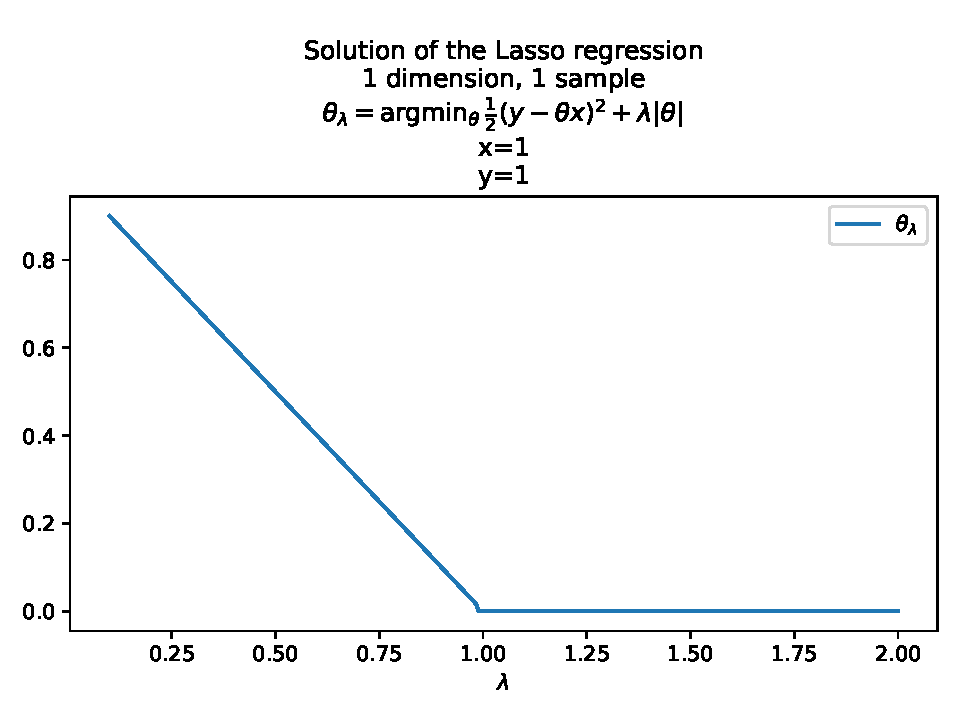
\includegraphics[width=1\textwidth]{lasso_regression_x_1_y_1}
    \caption{Solution of the one-dimensional Lasso estimator}
    \label{fig:lasso_regression_x_1_y_1}
\end{figure}

\section{\large\color{Blue}Solution}

Depending on the sign of $\theta$, and the values of $\lambda$ and $y$, the situation will be different. However, we need to keep in mind that we always have that $\lambda \geq 0$, as it is a regularization parameter.


\subsubsection{$\theta \geq 0$}%

    If $\theta\geq 0$, we have that

    \begin{equation}
	F_{\lambda}(\theta) = \frac{1}{2}(y-\theta)^2+\lambda \theta
    \end{equation}

    We can differentiate with respect to $\theta$, and

    \begin{equation}
	F_{\lambda}'(\theta) = -(y-\theta)+\lambda = \theta - (y-\lambda)
    \end{equation}

    In this case,

    \begin{itemize}
	\item If $\lambda \geq y$, then $y-\lambda \leq 0$, and we always have that $F_{\lambda}'(\theta)\geq 0$, the minimum on $ \mathbb{R}_+$ is attained for $\theta=0$, with value $\frac{1}{2}y^2$.
	\item If $\lambda \leq y$, then $y-\lambda \geq 0$, and we have that $F_{\lambda}'(\theta)\leq 0$ if $\theta\leq y-\lambda$ and $F_{\lambda}'(\theta)\geq 0$ if $\theta\geq y-\lambda$, the minimum on $\mathbb{R}_+$ is attained for $\theta = y-\lambda$, with value $ \frac{1}{2}\lambda ^2  + \lambda(y-\lambda) = \lambda (y - \frac{1}{2}\lambda) $ 
    \end{itemize}

\subsubsection{$\theta \leq 0$}%

    If $\theta\leq 0$, we have that

    \begin{equation}
	F_{\lambda}(\theta) = \frac{1}{2}(y-\theta)^2-\lambda \theta
    \end{equation}

    We can differentiate with respect to $\theta$, and

    \begin{equation}
	F_{\lambda}'(\theta) = -(y-\theta)-\lambda = \theta - (y+\lambda)
    \end{equation}

    In this case,

    \begin{itemize}
	\item If $\lambda \geq -y$, then $y+\lambda \geq 0$, and we always have that $F_{\lambda}'(\theta)\leq 0$, the minimum on $ \mathbb{R}_-$ is attained for $\theta=0$, with value $ \frac{1}{2}y^2$.
	\item If $\lambda \leq - y$, then $y+\lambda \leq 0$, and we have that $F_{\lambda}'(\theta)\leq 0$ if $\theta\leq y+\lambda$ and $F_{\lambda}'(\theta)\geq 0$ if $\theta\geq y+\lambda$, the minimum on $\mathbb{R}_-$ is attained for $\theta = y+\lambda$, with value $ \frac{1}{2}\lambda ^2  - \lambda(y+\lambda) = \lambda(-y-\frac{1}{2}\lambda) $ 
    \end{itemize}


\subsection{Applications}%
\label{ssub:Applications}

Let us consider some values of $y$ and plot the $\theta_{\lambda}$ as a function of $\lambda$.

\subsubsection{$y=1$}%
\label{ssub:$y=1$}

In this case:

\begin{itemize}
    \item If $\lambda \leq 1$,
	\begin{itemize}
		\item the optimal $\theta\in \mathbb{R}_+$ is $\theta_+ = 1-\lambda$ with value $\lambda (1- \frac{1}{2}\lambda)$.
		\item the optimal $\theta\in \mathbb{R}_-$ is $\theta_- = 0$ with value $\frac{1}{2}$.
	\end{itemize}

        Let us show that is $0\leq \lambda \leq 1$, then $ g(\lambda)=\lambda
        (1- \frac{1}{2}\lambda)\leq \frac{1}{2}$. We have that
        $g(\lambda)=\lambda-\frac{1}{2}\lambda^2$, hence
        $g'(\lambda)=1-\lambda\geq 0$. The maximum value of $g(\lambda)$ is
        thus attained in $\lambda=1$, and is equal to $ \frac{1}{2}$.

         Overall, we have

	\begin{equation}
	    \theta_{\lambda} = 1-\lambda
	\end{equation}
	and 
	\begin{equation}
	    F_{\lambda}(\theta_{\lambda}) = \lambda (1- \frac{1}{2}\lambda)
	\end{equation}
    \item If $\lambda \geq 1$,
	\begin{itemize}
		\item the optimal $\theta\in \mathbb{R}_+$ is $\theta_+ = 0$ with value $\frac{1}{2}$.
		\item the optimal $\theta\in \mathbb{R}_-$ is $\theta_- = 0$ with value $\frac{1}{2}$.
	\end{itemize}

	Overall
	\begin{equation}
	    \theta_{\lambda} = 0
	\end{equation}
	and 
	\begin{equation}
	    F_{\lambda}(\theta_{\lambda}) = \frac{1}{2}
	\end{equation}
	
\end{itemize}




\end{document}
